\documentclass[border=10pt]{standalone}

\usepackage{tikz}
\usepackage{tikzsymbols}
\usetikzlibrary{calc,patterns,shapes.geometric}

\def\centerarc[#1](#2)(#3:#4:#5){\draw[#1] ($(#2)+({#5*cos(#3)},{#5*sin(#3)})$) arc (#3:#4:#5);}

\begin{document}
	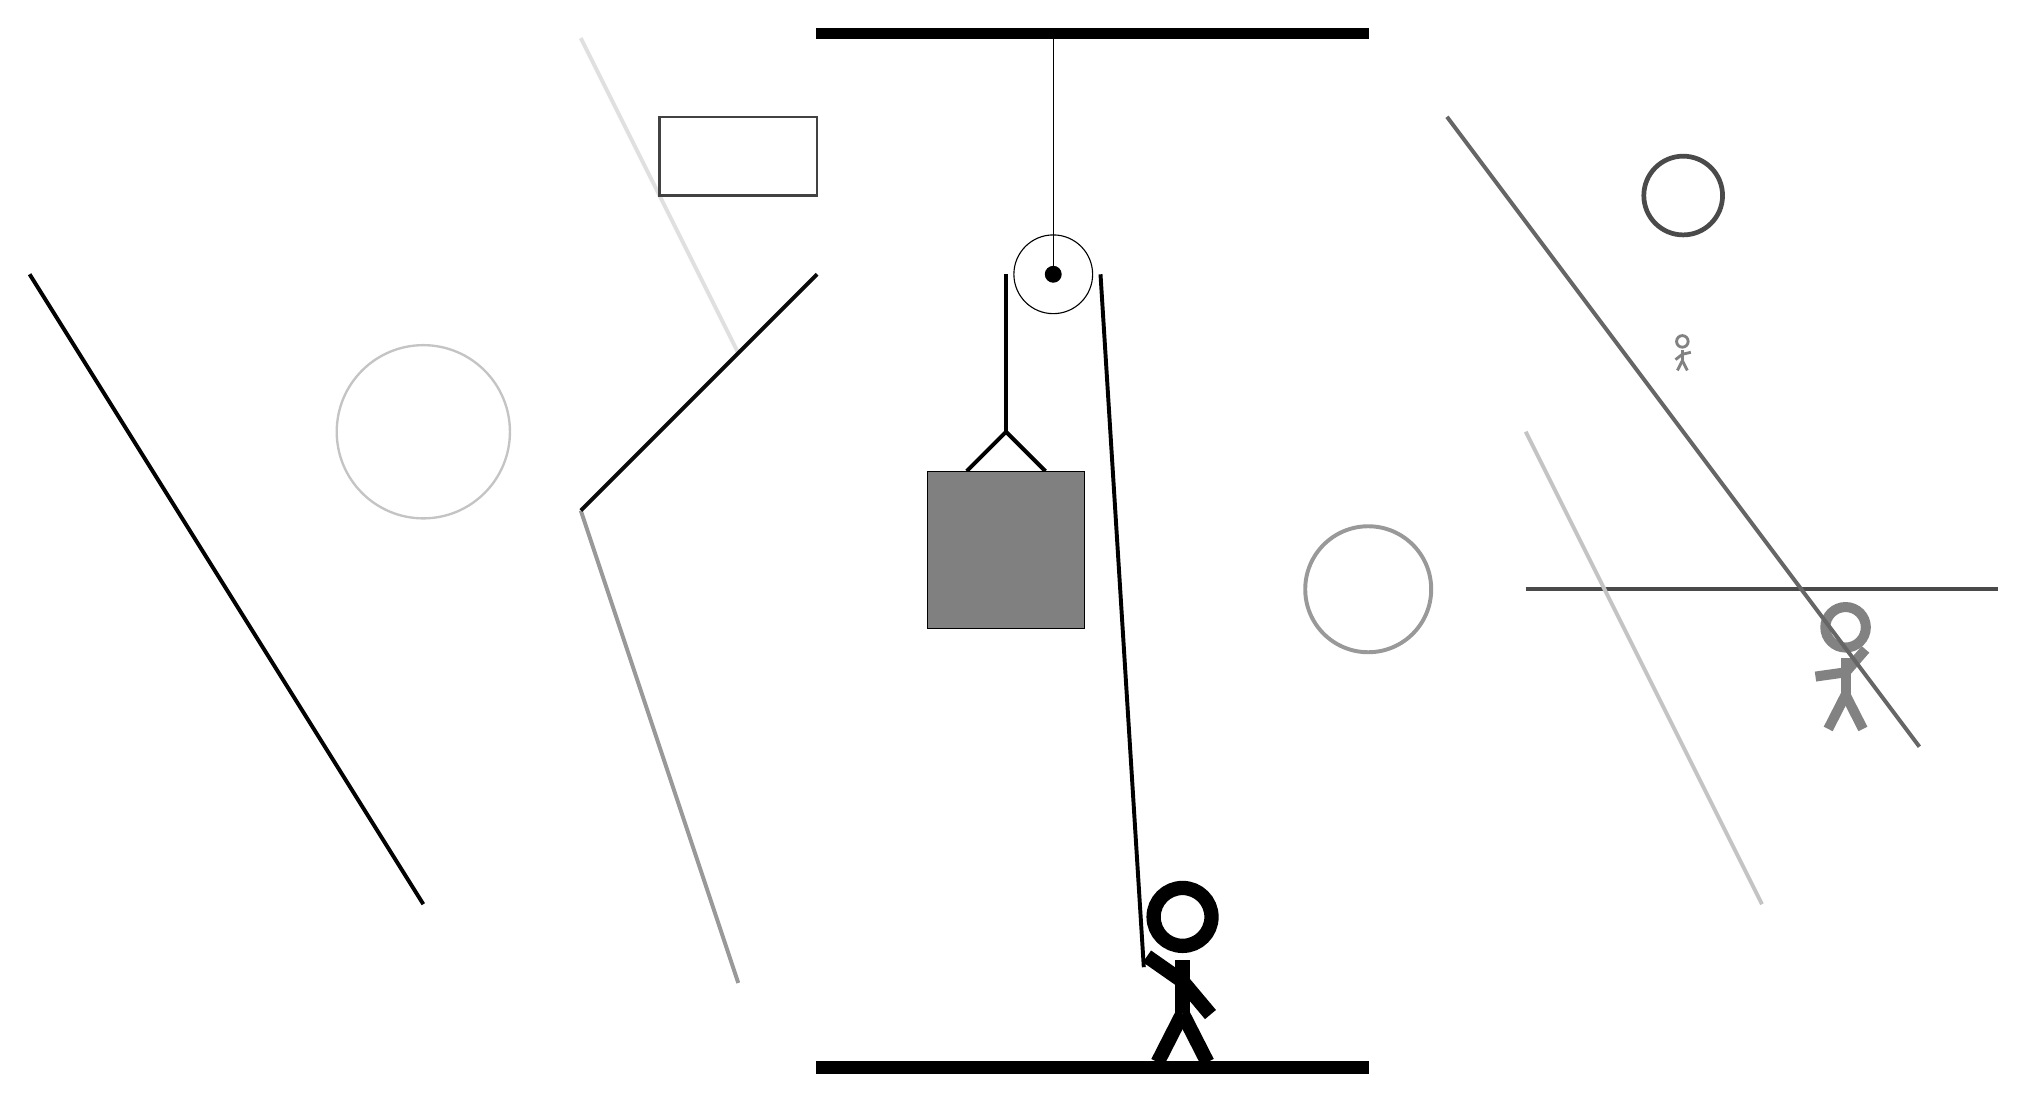
\begin{tikzpicture}
		%%%%% START %%%%%
		
		\draw[fill=black] (-2, 10) rectangle (5, 10.125);
		
		\draw[line width=0.5mm, color=black!40](-5, 4) -- (-3, -2);
		
		\draw[line width=0.3mm, color=black!73] (6, 10) rectangle (6, 10);
		\draw[line width=0.5mm, color=black!71](7, 3) -- (13, 3);
		\node[line width=0.5mm, color=black!49] at (11, 2) {\Strichmaxerl[7][8][49]};
		\draw[line width=0.5mm, color=black!12](-5, 10) -- (-3, 6);
		
		\draw[line width=0.5mm, color=black!99](-7, -1) -- (-12, 7);
		\draw [line width=0.6mm, color=black!71](9, 8) circle (0.5);
		\draw [line width=0.5mm, color=black!12](7, 3) circle (0.0);
		\node[line width=0.7mm, color=black!49] at (9, 6) {\Strichmaxerl[2][38][13]};
		
		\draw[line width=0.3mm, color=black!74] (-4, 9) rectangle (-2, 8);
		
		\draw [line width=0.3mm, color=black!23](-7, 5) circle (1.1);
		\draw[line width=0.5mm, color=black!96](-2, 7) -- (-5, 4);
		\draw [line width=0.5mm, color=black!40](5, 3) circle (0.8);
		\draw[line width=0.5mm, color=black!23](10, -1) -- (7, 5);
		\draw[line width=0.5mm, color=black!60](6, 9) -- (12, 1);
		
		\draw (1, 7) circle (0.5);
		\draw[fill=black] (1, 7) circle (0.1);
		\draw (1, 10) -- (1, 7);
		
		\draw[line width=0.5mm] (-0.1, 4.5) -- (0.4, 5.0) -- (0.9, 4.5);
		\draw[fill=black!50] (-0.6, 4.5) rectangle (1.4, 2.5);
		
		\draw[line width=0.5mm] (0.4, 7) -- (0.4, 5.0);
		\centerarc[line width=0.5mm](1, 7)(0:180:0.6);
		\draw[line width=0.5mm](1.6, 7) -- (2.15, -1.8);
		
		\node at (2.6, -1.9) {\Strichmaxerl[10][-35][-50]};
		
		\draw[fill=black] (-2, -3) rectangle (5, -3.15);
		
		%%%%% END %%%%%
	\end{tikzpicture}
\end{document}